\part{Exercice 9}

On pose $q = 1 - p$.

La probabilité que l'avion à deux moteurs arrive à destination est $P_A(D) = q^2 + 2pq = 1 - p^2$.

La probabilité que l'avion à quatre moteurs arrive à destination est $P_B(D) = q^4 + 4pq^3 + 6p^2q^2$.

On pose $f : p \mapsto (1-p)^4 + 4p(1-p)^3 + 6p^2(1-p)^2 - 1 + p^2$.

\danger erreur de calcul probable.


$\forall p \in [0,1],\,f(p) = 3p^4 - 4p^3 + p^2 = p^2\underbrace{(3p^2 - 4 p + 1)}_{\mathclap{\Delta = 16 - 4 \times 3 \times 1 = 4}}$

\begin{center}
	\begin{tikzpicture}
		\tkzTabInit[nocadre]{$p$/1, $f(p)$/2}{0,$\frac{1}{3}$,1}
		\tkzTabLine{,+,z,-,z}
	\end{tikzpicture}
\end{center}

